\vspace{1cm}
\section{Zwei und Mehrtore}
\subsection{Komplexe Wellenamplituden}
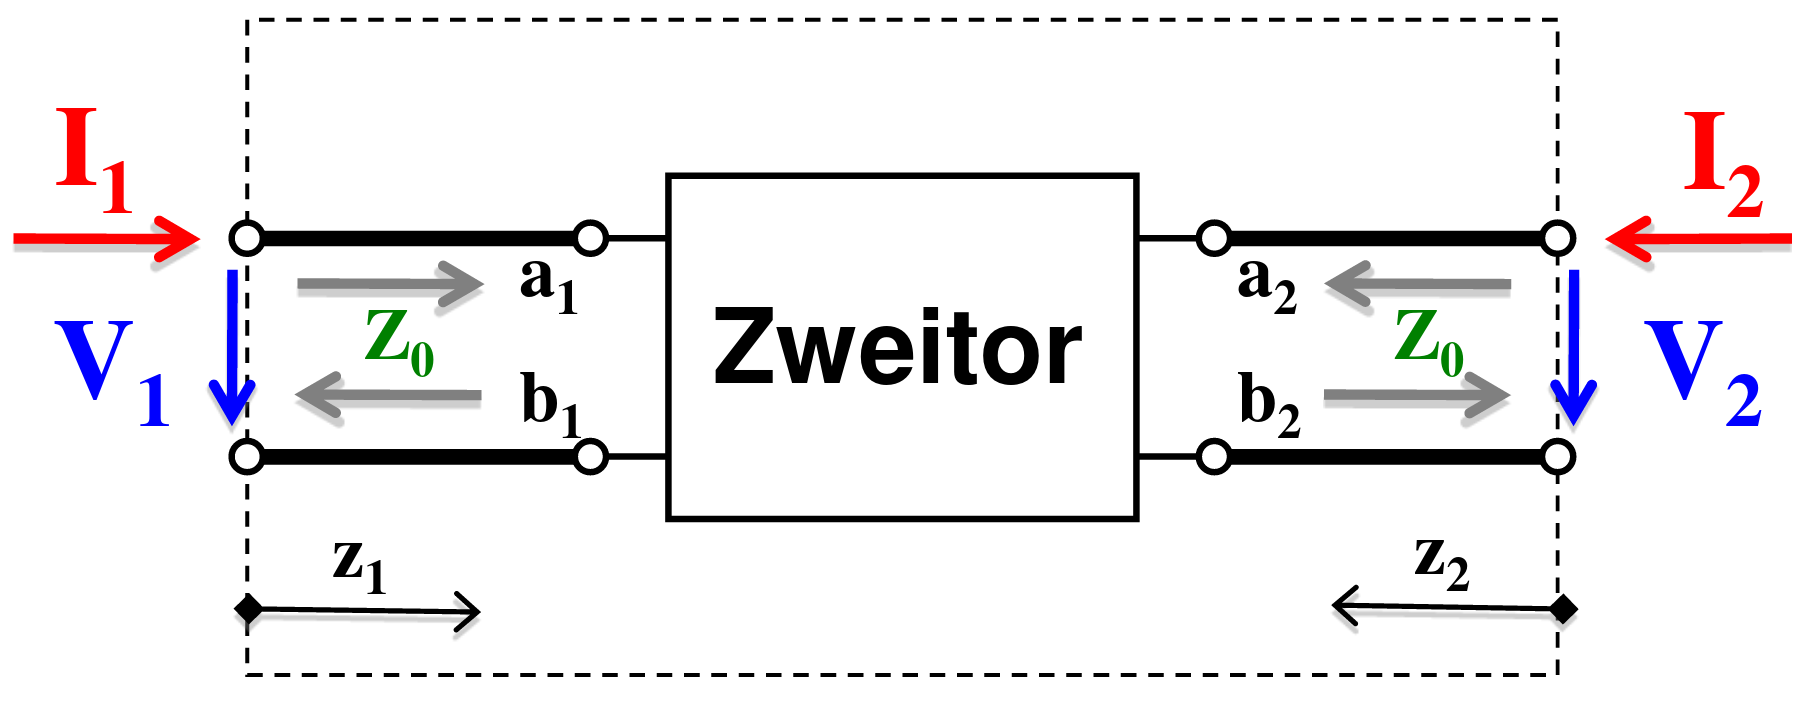
\includegraphics[width= 0.35\paperheight]{content/fuw/pictures/hf_zweitor.png}
    \begin{itemize}
        \itemsep0pt
        \item Verwendung von Strom/Spannung wenig sinnvoll, wegen der starken Empfindlichkeit zur Leitungslänge
        \item \textit{Stattdessen:} komplexe Amplituden $a$ und $b$
        \item Hinlaufende Welle $a_1$ bzw. $a_2$
        \item Rücklaufende Welle $b_1$ bzw. $b_2$
        \item Definition der Wellenamplituden:
        \begin{align*}
            a_k  = \dfrac{1}{2\sqrt{2 Z_0}}(U_k + Z_0 I_k)\\
            b_k  = \dfrac{1}{2\sqrt{2 Z_0}}(U_k - Z_0 I_k)
        \end{align*}
\end{itemize}
\subsection{Streuparameter}
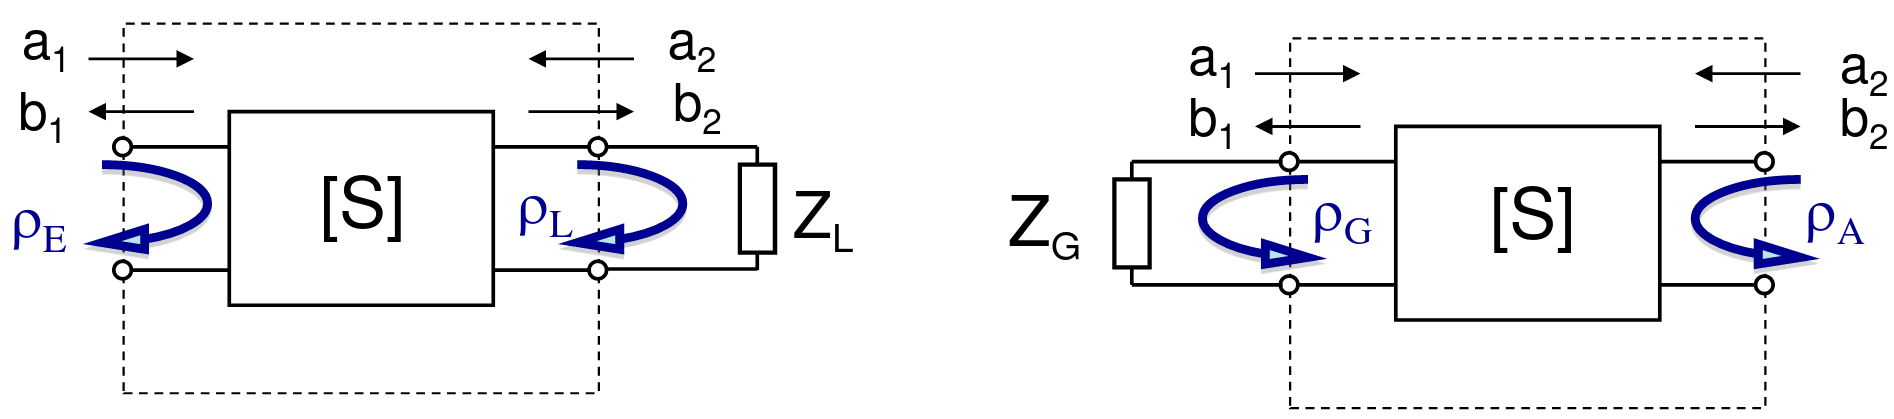
\includegraphics[width=0.35\paperheight]{content/fuw/pictures/hf_zweitor_reflektion.png}
\begin{itemize}
    \itemsep0pt
    \item Streuparameter der $S$-Matrix
    \item \textit{Allgemein:} \(\underline{b} = S \underline{a}\)
    \item Für ein Zweitor:
    \begin{align*}
        b_1 &= S_{11} a_1 + S_{12} a_2\\
        b_2 &= S_{21} a_1 + S_{22} a_2
    \end{align*}
    \item \textbf{Anpassung:} allseits reflexionsfrei\\
        \(s_{ii} = 0, \;\forall i \in (1;\; \mathrm{dim}(S))\)
    \item Eingangsreflexionsfaktor\\
        \(\rho_E = \dfrac{b_1}{a_1}; \;\;\; \rho_L = \dfrac{a_2}{b_2}\)
    \item Ausgangsreflexionsfaktor\\
        \(\rho_A = \dfrac{b_2}{a_2}; \;\;\; \rho_G = \dfrac{a_1}{b_1}\)
    \item \textbf{Reziprozität} (Übertragungssymmetrie): \(S = S^\top\)
    \item \textbf{Verlustfreie} n-Tore ($S$ unitär):\\
        \(\sum^n_{i=1} |b_i|^2 = \sum^n_{i=1} |a_i|^2 \implies S^\top S^* = I\)
    \item Verlustfreies, reziprokes, allseits angepasstes 3-Tor\\
        \(\implies\) nicht realisierbar
\end{itemize}

